
\chapter{Introduction}

\section{Background}

Political conflicts are complex. This is the expected opening in a dissertation such as this, but it is nevertheless true. They involve cooperation and competition between multiple actors who differ from one another in their capabilities, their objectives, and even their decisionmaking processes. Furthermore, these actors themselves are often complex -- they are generally political entities (primarily states, though increasingly non-state groups as well) which are ultimately composed not only of individuals but of procedures, institutional memory, and other emergent characteristics. To paraphrase an old joke, it's complexity all the way down.

Much of the study of political science and international relations seeks, naturally enough, to reduce this complexity, and does so with a wide variety of methodologies and tools. General theories of how actors make decisions and interact, derived from and applied to case studies of particular events, are as old as the discipline itself. More recently, such studies have encompassed not just state-level power, security, and institutions, but the incentives and behaviors of sub- and non-state actors, and even the psychological biases of individual decisionmakers. Quantitative and statistical methods have become the mainstays of the discipline, offering powerful tools to identify regularities and test theories in datasets of actor properties, relationships, and events. Game theory grew in part out of Cold War-era security analysis and policymaking. It has provided a language that can formally describe and analyze strategic interactions, and yielded powerful concepts such as the notion of a Nash equilibrium, and stylized, insight-generating models such as the Prisoners' Dilemma.

These lines of research are often somewhat disconnected from one another. Many grand theories are extremely general, and can only be explored via detailed case studies, or statistically tested one narrow implication at a time. Similarly, psychological theories require notional lab experiments or detailed archival sources on the beliefs and actions of key individuals in a particular crisis. Game-theoretic models are generally relatively abstract, and rarely intended to be applied to data to generate specific testable predictions. Statistical models have gained prominence in part because they can be used to operationalize and test hypotheses developed from various theories. These tests require appropriate and accurate empirical data, which is often difficult to collect, and many statistical tools do not account for the interdependence between cases in the dataset. Statistical models are generally capable of accounting for some top-level outcome variable, but rarely attempt to capture the interactions and decisions by which that outcome was reached; they provide outcome validity, but not necessarily process validity. 

Comparative analysis is an important tool, frequently applied across different methodologies. Tables reporting the results of multiple regressions side by side are a common sight in quantitative studies: by comparing the fit and coefficients of several statistical models, we can evaluate which one has more explanatory power, and whether hypothesized relationships in fact occur in the data. Case studies may also be used to compare multiple theories, examining a single case in detail and identifying which events and processes can be explained by (or contradict) each, or reviewing sets of cases together and locating meaningful commonalities. Many theories and models have limited explanatory power on their own, making it hard to assess them without a basis for comparison. This is particularly true for more general theories that abstract away from the actor- and situation-specific details that often drive a great deal of interactions. By comparing two or more theories side by side, we can assess which one does a better job at explaining the cases or data in question.

Agent-based models (ABMs) are a powerful tool for studying complex systems in general \citep{miller_2007}, and appear particularly suitable to apply to international relations \citep{cederman_1997}. By definition, ABMs consist of independent actors (agents) interacting with one another and with their environment. The agents are programmed with particular behaviors, which may include, for example, extremely simple \emph{if-then} rules, operationalizations of particular qualitative theories, or complicated optimization methods. Since models are often implemented primarily at the agent level, they can be used to identify emergent, aggregate phenomena arising from the simulated lower-level interactions. Though ABMs have never entered the mainstream of international relations research, there have been several attempts to build and study such models. Many of these attempts \citep[e.g.][]{axelrod_1997,cederman_1997,min_2002} have involved relatively abstract, notional systems. Such models attempt to capture a few key aspects of the behavior of countries, and use these simulated states to grow an international system `from the bottom up,' exploring how well the hypothesized behaviors lead to the emergence of properties observed in reality. Another set of models explicitly attempt to model real-world actors, and are intended for forecasting and policy support \citep[e.g.][]{taylor_2008,abdollahian_2006}. These models, in contrast typically do not attempt to test specific theories, though it is hard to determine for certain as they are almost universally proprietary.

This dissertation will attempt to demonstrate that agent-based modeling may be used in a different way, and can serve as a bridge between several of the other methodologies and paradigms \citep{axelrod_2006}. Such models need not be confined to notional worlds, but can be applied to real-world interactions as well. Empirical application, in fact, offers a way to directly compare the theories of interaction and decisionmaking that the models are based on. In order to demonstrate this, I reimplement two prior formal models of international conflict as agent-based models, arguing that their structure is already amenable to such conversion. Elements of the models are modified, endowing the agents with alternative internal models of decisionmaking; I then instantiate different model variants with the same input data, in order to directly compare their behaviors and outputs. By comparing these outputs' relationships to empirical, historic data, I directly determine which model variant best explains and predicts the observed data.

\section{Current Methods in Conflict Modeling}\label{current-methods-in-conflict-modeling}

\subsection*{Case Studies}
% AC: Example of such histories?
Histories have described the decisionmaking process of key actors in international interactions since long before history was an established academic discipline, and international relations scholarship has long drawn on these descriptions to generate general theories. Modern scholarship has extended this technique into the case study, with the researcher methodically analyzing primary and secondary descriptions of an incident or set of incidents. Such analysis may involve attempts to tease apart commonalities in order to build a new theory; however, more often it involves applying a particular prior theory to the cases in question, examining where the theory can or cannot provide an adequate explanation for the observed events \citep{george_2005}. In ``The Essence of Decision,'' \citet{allison_1999} provide a key demonstration of this methodology, laying out three theories of political decisionmaking and analyzing the Cuban Missile Crisis through the lens of each in turn, highlighting decisions that can adequately be explained by one or more of the theories, and (more importantly), decisions which appear to contradict one theory but can be explained by another. Similarly, \citet{jervis_1976} lays out a series of psychological models expected to drive the behavior of individuals and small groups of decisionmakers, and presents historic evidence that such theories indeed explain events observed across multiple past crises. \citet{kaufmann_1994} focuses on one particular case, and uses it to test a similar psychological model against the alternative theory that the decisionmakers were acting rationally, demonstrating that the proposed biases explain divergences between actors that have no purely rational explanation.

There can be little doubt that case studies provide a vital tool for understanding how decisions are actually made and identifying the strengths and weaknesses of existing theories. However, case studies are limited by the need for detailed historical or archival information. \citet{allison_1999} rely on transcripts of discussions among the American leadership during the Cuban Missile Crisis and detailed records of American and Soviet military deployments, while \citet{kaufmann_1994} relies on letters between the key leaders to identify when, and in response to what, each changed his opinion. This requirement makes it difficult to falsify theoretical predictions: for example, an earlier edition of ``Essence of Decision'' \citep{allison_1971} made theory-driven predictions as to the structure and process of the Soviet decisionmaking, which were only proven to be incorrect decades later, when the fall of the Soviet Union made the relevant historic documents available. Furthermore, case studies require `cases' -- for our purposes, crises or conflicts which come to the attention of the analyst. However, a theory may correctly predict many instances where no conflict occurs, and if indeed no conflict occurs then no case for examination will be generated. \citet{achen_1989} further argue that case studies alone are insufficient to truly test theories, as they lend themselves too readily to highlighting case-specific exceptions and cannot adequately measure the power of a theory across multiple cases. Such rigorous comparison, they argue, can only be done using statistical analysis.

\subsection*{Statistical Models}\label{statistical-models}

Statistical and econometric modeling have become the most common methodology in international relations research \citep{colgan_2016}. In general, researchers will develop a qualitative theory or take one from prior literature, and operationalize it as an econometric model attempting to explain a dependent variable (e.g. the outbreak of war) in terms of several independent variables (such as the system of government and military strength of the belligerents). The researchers then fit the model to an appropriate dataset. If the model fits the data well (e.g. high $R^2$, low mean squared error), and the coefficients are statistically significant and have the hypothesized signs and magnitudes, this is taken as evidence of the theory's validity. Alternatively, the coefficients that are determined to be significant can be used to develop new theories which account for the observed relationship. A model can be further tested by applying it outside of the sample used to fit it, either by withholding a subset of the data for testing, or (better yet) applying it to future cases outside the dataset altogether.

An important reason that statistical analysis has become a core research tool is that ``it basically works,'' \citep{schrodt_2004}. There are many, many examples of statistical models applied to international relations in general, and to conflict in particular. For example, \citet{bremer_1992} tests numerous factors hypothesized to make wars between dyads of states more likely, showing that many factors are less important than previously thought; while \citet{hagan_1994} estimates how states' domestic politics affect their propensity to engage in wars. \citet{wayman_1994} review multiple statistical tests of the qualitative predictions of Realist theories, arguing that they are insufficient to explain much of the international system. Such models can be applied specifically to forecasting. The work of \citet{goldstone_2005} with the Political Instability Task Force (PITF) can generate accurate predictions as to which countries will experience internal instability over a two-year period, and is used for government planning and policymaking. Similarly, \citet{ward_2013} uses statistical methods to generate regularly-updated forecasts for the outbreaks of civil wars. More recently, such models have been applied not just to the outbreak of conflicts but to the counts of specific events. For example, \citet{yonamine_2013} applies statistical models originating in finance to predict the intensity of conflict in Afghanistan, while \citet{brandt_2011} propose a general time-series model for the number of individual events within any given ongoing conflict, with an initial focus on Israeli-Palestinian interactions.
 
While the statistical approach may indeed provide what \citet{schrodt_2004} refers to as `outcome validity', by and large it is not intended to provide `process validity'. \citet{goldstone_2005}, for example, can predict where instability will occur, but not which particular actors will initiate or be involved in it. Furthermore, one of the variables with the greatest predictive power for internal political instability is infant mortality \citep{goldstone_2005}. Yet high infant mortality is not directly the cause of most instability, nor is it exogenous to the system as a whole \citep{marshall_2008}. Similarly, though many statistical analyses \citep[e.g.][]{maoz_1989,thompson_1997,gartzke_2007} have confirmed that democracies are less likely to go to war with one another (so-called democratic peace theory), they do not offer a consensus as to why this is the case.

These difficulties point to another challenge facing the use of statistical techniques. Political interactions are generally believed to be strategic: actors on all sides can anticipate the other actors' likely responses to possible actions they may take, and make their own decisions accordingly. These strategic considerations can lead to censoring in the data we observe in the world \citep{smith_1999}, and to non-linearities in the relationship between input variables and expected outcome \citep{signorino_1999}. To provide a simplified example: if countries are highly likely enter wars when the balance of forces is above a certain threshold, and highly unlikely to otherwise, the population of observed wars would only include cases where the actors' force ratio falls into the range between these thresholds. However, a logistic regression predicting the probability of war from both sides' forces would not detect those sharp break-points. 

\subsection*{Game Theory}\label{formal-game-theoretic-models}

In order to overcome the challenge of analyzing data generated from strategic interactions, \citet{signorino_1999} and \citet{smith_1999} independently proposed statistical models explicitly informed by game theory. Game theory is the mathematical study of interactions (games) between two or more `players' whose payoffs depend not only on their own choices but those of the other players as well. Much of modern game theory was developed explicitly for the study of international conflict \citep{myerson_2009}, particularly by researchers at the RAND Corporation \citep{gates_1997}. Game-theoretic or formal models are widely used in political science, where they are used to represent conflict \citep[e.g.][]{powell_2006}, negotiation \citep[e.g.][]{brams_2003}, elections \citep[e.g.][]{coughlin_1981} and more. \citet{gintis_2015} have even recently proposed to apply game theory as a foundation to an attempt to derive a mathematical model for all of human society.

Statistical models explicitly incorporating game-theoretic elements are still relatively rare. Many formal models are not intended to represent specific historically-situated events or interactions; they are notional and abstract, meant to capture common characteristics encountered in multiple cases \citep{snidal_1985}. By solving the models analytically and identifying and parameterizing their equilibria, researchers can identify general theories of strategic behavior and interaction. There have also been several attempts to apply game-theoretic models to empirical data in addition to the statistical models referenced above. \citet{bdm_1992} apply an extensive-form model of crisis escalation to historic dyads, an effort extended substantially by \citet{bennett_2000}. \citet{bdm_1994,bdm_1997,bdm_2002} presents a game theory based model of negotiation and coercion which is explicitly intended as a forecasting tool. These models will be the focus of this dissertation, and so will be described at length later. Additional examples include \citet{tsebelis_1988} proposing a multilateral formal model to explain the outcome of French elections, and \citet{metternich_2013} using equilibria in a network-based model to explain the intensity of opposition group activity in Thailand.

A fundamental assumption of game theory is that the players are rational, which here has a formal definition: that they take actions in order to maximize their utility, aware of and taking into account the other players' rationality. This leads to equilibria, the strategies leading to the best result players can achieve while assuming that all other players are playing their equilibrium strategy as well. The assumption of rationality allows the modeler to analyze and solve the game, as it implies that the actors are conducting the same analysis themselves, and are acting accordingly.

The rationality assumption is, not surprisingly, the source of much of the criticism of game theory. Behavioral economics has shown that human players' deviations from perfect rationality are not merely a white-noise error term, but systemically driven by psychological \citep{tversky_1981} and cultural \citep{henrich_2005} factors. Recently, behavioral game theory has begun to incorporate such insights into game-theoretic models \citep{camerer_2003} in order to model the behavior of players who are not formally rational. Much like individual humans, organizations may not be rational either, and their decisionmaking is characterized by their own heuristics \citep{march_1993} and systemic biases \citep{shapira_2002}. While defenders of the rationality assumption such as \citet{friedman_1953} argue that actors need not be procedurally rational \citep{simon_1976} for the equilibrium outcomes to serve as useful predictors, both statistical analyses \citep{bennett_2000} and detailed case studies \citep{allison_1999,kaufmann_1994} suggest that real decisionmaking deviates systemically from the formal predictions. In laying out an agenda for the future of game theory research, \citet{fudenberg_2010} suggests a relaxation of this assumption is necessary to allow models to capture the full range of observed behaviors.

\subsection*{Computational Methods}\label{computational-methods}

Computational methods are not a well-defined family of methodologies like the ones discussed in the previous sections. I use the phrase very broadly, to mean any method which in practice relies on a computer to implement, and does not fall into the categories above. In practice, there are roughly three broad subcategories of computational methods: dynamical systems models, machine learning, and agent-based models.

Dynamical systems models represent components of interest as stocks and flows connected to one another and often exhibiting feedback loops \citep{gilbert_2005}. While many such models can ultimately be represented as systems of differential equations, in practice their complexity often requires them to be approximated numerically. Early dynamical systems models relevant to international relations include the \citet{lanchester_1916} models of ancient and modern warfare, and the Richardson arms race model \citep{rapoport_1957}, both of which emerged from the First World War. The introduction of computers, and the growth of interest in systems theory, led to computational systems dynamics models of international relations, such as the Globus Model \citep{bremer_1987}. The Richardson model has been widely tested, and found to be insufficient to explain the dynamics of arms acquisition even between pairs of well-established rivals \citep{dunne_1999}. This approach in general appears to have fallen out of favor in recent years.

Machine learning is, essentially, an extension of statistical methods to leverage expanded computational resources, and this is largely how it has been used in political science. \citet{goldstone_2005} experimented with using methods such as neural networks or Random Forests \citep{breiman_2001} before returning to the logistic regression. \citet{schrodt_1997} used a hidden Markov model to predict the dynamics of conflict in the Middle East, and presents several other approaches (decision trees, neural networks and sequence matching) as prediction methods as well \citep{schrodt_2004} . While these approaches allow for more sophisticated relationships between predictors and outcomes, they suffer from many of the same problems as the more traditional statistical approaches, particularly the `process' versus `outcome' validity distinction. Furthermore, these approaches often trade accuracy for interpretability, resulting in models with strong predictive power but which cannot be directly mapped to a qualitative theory.

% AC: Can ABMs be used to build theories, i.e. Axelrod's Third Way.
Finally, and most relevantly for this dissertation, are agent-based models (ABMs). In these models, each actor is represented by a discrete agent, and the agents interact with one another within some sort of environment. In general, ABMs are operationalizations of a particular qualitative theory from which the agent behaviors are derived. The agent behavior may consist extremely simple rules such as tit-for-tat \citep{hudson_2004,axelrod_1980}; more complicated heuristics \citep{cederman_1997}; artificial intelligence-derived planning algorithms \citep{taylor_2008}; or adaptive behavior \citep{hoffmann_2005,rouleau_2011}. The level of abstraction of these ABMs also varies widely. Many are `artificial societies' \citep{epstein_1996}, testing how simple assumptions and behaviors lead to the emergence of key features of the international system. For example, \citet{cederman_1997} models an international system as consisting of political actors on a square grid, using simple theory-derived heuristics to decide whether to go to war with their neighbors, and demonstrates how this leads to state and empire-like entities, and later \citep{cederman_2003} under what conditions the power-law distribution of conflict scales \citep{richardson_1948} arises. Other models are intended explicitly for forecasting and policy analysis. For example, \citet{taylor_2008} describe a generic (and non-public) model of political conflict, called the Power Structure Toolkit (PSTK), meant to allow subject-matter experts to generate and test scenarios with specific agents endowed with heterogeneous capabilities and goals. The objective of this model is as a decision support tool, rather than a test of any particular theories or hypotheses.

Abstract ABMs serve similar purposes to formal models, presenting relatively sparse theory implementations in order to yield general insights. By relaxing the requirements for perfect rationality and analytic tractability, they can describe richer interactions with a greater number of actors, and explore the models' properties and the emergent phenomena they may give rise to. Such ABMs must qualitatively ground their assumptions, and require additional analysis due to the number of moving parts to ensure that their results are robust, and not merely artifacts of the model. Something as simple as the agent activation order may have profound and unanticipated impacts on the model results \citep{comer_2014}. Furthermore, there is not always a clear mapping between the outputs of an abstract ABM and empirical data.

Empirical ABMs appear to be even less common in international relations. Such models often require significant amounts of data, or assumptions when necessary data is missing. Similarly, the more complicated the agent behavior, the more coding is required, adding to the assumptions, the parameters to be estimated or explored, or potential points of failure. These requirements help suggest why many empirical ABMs of international relations appear to be primarily developed in the commercial or government sectors, including \citet{taylor_2008}, \citet{abdollahian_2006} and \citet{chaturvedi_2000}.

\section{Research Contribution}

In this dissertation, I develop the use of agent-based modeling as a methodological bridge between several of the paradigms and tools I have described above. The methodology I propose is illustrated in Figure \ref{fig:architecture}: I begin by implementing established, well-validated models as ABMs, and introduce changes in particular sub-models in order to generate several different model variants. Empirical data for a particular starting point (such as alliances and material capability data, described in Section \ref{data-sources}, below) is used to generate sets of agents, which instantiate all the model variants. Multiple simulation runs then generate several output datasets associated with each model variant. By statistically comparing these outputs to empirical data on the corresponding time period, I can assess which model variant has the most explanatory power, which in turn offers evidence for the hypotheses the variant is based upon.

\begin{figure}[h!]
	\figSpace
    \centering
	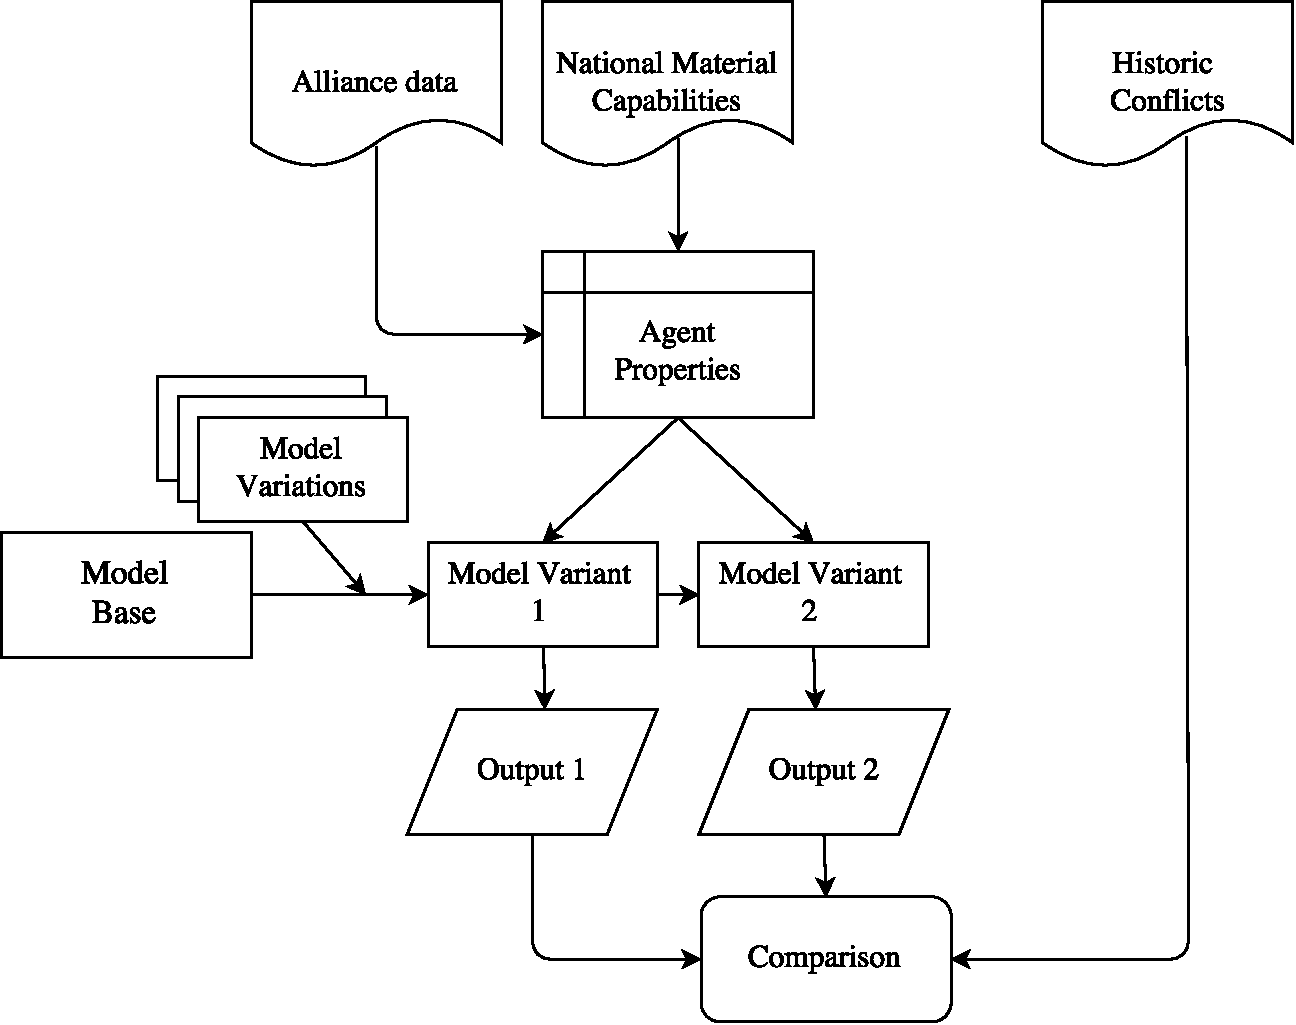
\includegraphics[width=0.75\textwidth]{figures/ModelFlowChart}
    \caption{Modeling Methodology}
    \label{fig:architecture}
    \figSpace
\end{figure}

The two models I reimplement and adapt are the International Interaction Game (IIG) \citep{bdm_1992,bennett_2000}, and the Expected Utility Model (EUM) \citep{bdm_1994,bdm_1997,bdm_2002}. Though I did not intend to focus on the works of Bruce Bueno de Mesquita in particular, these two models are among the few game-theoretic models of international relations that have been instantiated with data intended to capture real-world scenarios and have had their results compared to empirical data for those scenarios. Both are also amenable to implementation as ABMs: they consist of unitary actors, interacting with each other in discrete steps within a broader environment of other actors. Both are ultimately models of the actors' decisionmaking, and keep many other factors (such as the actors' coercive capabilities) exogenous. Yet both also make it possible to separate the actors' actions from the process by which they decide on them. This allows me to replace the original decisionmaking models with alternative ones based on different theories, repeat the same interactions, and see where the results correspond or diverge.

I implement both models using an object-oriented approach, keeping the sub-models as separate as possible. Each model has an overall World class which contains the agents, schedules their activation, and collects data on their interactions, where each World object is a particular model instantiation, used for one model run. The World class may also have inner classes for different sub-models. The agents are implemented such that they are comprised of two classes: the outer class stores the agents' public, common-knowledge properties, and sends and receives the interactions to the world and the other agents; the inner class controls the actual decisionmaking, storing internal, private properties and implementing methods for selecting among possible choices. This architecture allows for a clear separation between the interaction model and the decisionmaking model, and facilitates the substitution of different decision models between model instantiations.


For each model, I explore sub-model and decisionmaking variants anchored in different theories. As a baseline, I attempt to replicate the original models, and implement the  rational decisionmaking assumption they incorporate. I use the International Interaction Game to focus on agent decisionmaking, and implement two new agent models. One is driven by the idea that states, the agents in the model, make decisions using standard operating procedures \citep{allison_1999,levy_1986} which are updated based on simple feedback from past interactions \citep{steinbruner_1976}. The second model adds organizational memory, which the agents use to store the lessons learned from each previous interaction \citep{march_1993}; when facing a new interaction, the agents draw on the lessons of the most analogous past case \citep{khong_1992,schuman_1992}. Within the Expected Utility Model, I focus on the model's theory of coercion: embedded in the original model is an assumption that actors can use their power to directly impose their preferences on others, rather than simply inflict costs if their demands are not met. I implement and test a variant which brings the model in line with the understanding of coercion described by \citet{schelling_1966}. Other variants I implement bring the agents' risk acceptance sub-model in better line with Prospect Theory \citep{kahneman_1984,mcdermott_2001}, test the effect of the sequence of agent actions, and allow the agents to attempt to balance between potential threats.

Both the IIG and EUM have been applied to explain historic international conflicts, by attempting to use the models to predict the conflicts using earlier data. In \citet{bdm_1992} the IIG is applied to European country dyads from the years 1816-1970, which \citet{bennett_2000} extended to all global dyads between 1816 and 1992. Similarly, \citet{bdm_1998} instantiates the EUM with data on world and regional powers in 1948, and attempts to predict the course of the Cold War between the United States and Soviet Union. In both cases, the models' output is compared to data on the corresponding actors and period, with the similarity between them provided as empirical evidence that the models are effectively capturing relevant elements of the real world. Importantly, \citet{stokman_1994b} directly compare the outputs of early EUM implementation \citep{bdm_1994} with those of another model, the \citet{stokman_1994} Logrolling Model, which is instantiated with the same input data as the EUM but implements very different theoretical assumptions -- namely, that outcomes are reached via multi-issue compromises rather than coercion. I apply a similar methodology, and extend it in two ways. For each model variant, I run multiple instantiations in order to generate a distribution of outcomes which I can describe and explore. I also investigate the application of the EUM to machine-coded high-resolution political event data: to the best of my knowledge, the first such application. By comparing the output of each model to the empirical data, I can not only assess their fit individually but compare them to one another. If one model variant generates outputs which fit the empirical data better than another, this is evidence that the theories the variant implements have more explanatory and predictive power than the ones the other is based on. Similarly, if two variants have similar predictive power, it suggests that neither is necessarily better than the other.

Simply attempting to reproduce the results of previous models can be a valuable test, and provide a new perspective on the previous results (and indeed, in Chapter 3 I discuss the implications of failing to reproduce prior results). Additionally, this research provides several novel contributions. By anchoring agent-based models to accepted and well-studied models in international relations, I demonstrate that ABMs are not necessarily a separate and alien methodology in the discipline, but can be utilized as an extension to established research tools. In fact, as I will argue in Chapter 3, the EUM appears to be best understood as an ABM itself rather than a formal game-theoretic model. Furthermore, ABMs can implement theories of behavior which heretofore have been difficult to examine outside of resource-intensive case studies, allowing them to be tested statistically and comparatively on large-scale data.To summarize several conclusions, I find that non-rational theories have similar explanatory power to the theory of rational behavior, and that the \citet{schelling_1966}-based coercion sub-model yields better predictions in the EUM than the original version.

This research also advances the discipline of agent-based modeling itself in several ways. It demonstrates the value of designing models to be modular, in order to facilitate experiments incorporating different sub-models but controlling for other factors. It further demonstrates how such models can be anchored to real data, and how such data can be used to comparatively test the explanatory power of model variants, and the theories they operationalize. As I argue in Chapter 3, this is particularly important when models are not simply operationalizations of previous supported theories, but are themselves a new theory or hypothesis about the system being modeled. In this way, it extends \citet{epstein_2008}, utilizing ABMs for prediction not as a way of knowing the future but as a test of the underlying theory. 

Chapter 2 represents, to the best of my knowledge, the first application of reinforcement learning to a multi-agent model of agents dyadically playing an extensive-form game -- a narrow combination, to be sure, but one with relevance that likely goes beyond international relations. Indeed, though my substantive focus here is on international relations, the overall methodology of extending formal models into agent-based ones, implementing different sub-model variants, and testing them comparatively against empirical data, is likely applicable across other social science fields as well. This also contributes to the predictive game theory research agenda presented by \citet{fudenberg_2010}.

\section{Data Sources} \label{data-sources}

An important feature of the work in this dissertation is that it utilized historic, real-world data, both to provide the model inputs and to test the outputs. Several data sources will recur across chapters, and are thus worth examining in detail.

The majority of the datasets I use here originate from the Correlates of War (COW) project. This project is an informal collaboration of scholars who since 1963 have been facilitating the collection and dissemination of datasets useful for understanding wars and their causes \citep{cow_2016}. These datasets have become a primary tool in the quantitative study of conflicts, and of international relations more broadly. While there are several more detailed and specific datasets of interstate relationships \citep[e.g.][]{hendrix_2013,raleigh_2010}, there are no others with comparable breadth of scope. Applying the COW datasets to the computational models I present here is particularly fitting. In the first paper summarizing the project's early years, \citet{singer_1972} described the project's long-term ambitions: 
\begin{displayquote}
``[T]he natural next step would be [the conversion of analytical sub-models] to computerized, dynamic form. Then, by representing the most promising and powerful of these limited models as sub-routines of an ultimately integrated large-scale computer model, we can move to parameter estimation and sensitivity testing in a particularly effective fashion.''
\end{displayquote}

The first dataset used to derive inputs across all three chapters is the Formal Alliances dataset \citep{singer_1969,gibler_2009}. This dataset collects formal, written defense-oriented agreements between pairs of countries, including the dates that each agreement started and ended. Information on these treaties is collected from a variety of historical sources \citep{gibler_2004} and coded manually into several categories, with a spot-checking procedure used to ensure consistent coding. The most recent version of the data codes four categories of alliances, from defensive pacts requiring one party to intervene militarily if the other is attacked, to ententes which may merely pledge consultation when one party faces a crisis. 

In the models I present here, alliance data is generally not used directly -- that is, states are not necessarily assumed to come to the aid of allies they have defensive pacts with, for example. Instead, the models follow the approach introduced by \citet{bdm_1975} and treat alliances as indicators of states' unobserved interests. The more similar the sets of alliances of two states (their alliance portfolio), the closer their interests are considered to align. This similarity is estimated via Kendall's rank correlation coefficient (Kendall's tau-b) \citep{abdi_2007}.

The next dataset is the National Material Capabilities (NMC) \citep{singer_1972,singer_1988}, an estimation of states' `hard power' \citep{wilson_2008}, their military and coercive capabilities, for each year. The NMC data consists of six indicators: population size, urban population, energy consumption, iron and steel production, military expenditure, and number of military personnel. These indicators are then aggregated into a single Composite Index of National Capability (CINC) by averaging each state's share of each indicator for all states in the dataset for that year. This normalizes the data across the different units of measurement, and gives equal weighting to each indicator. It also means that CINC provides a measure of relative strength, which is only valid within a particular year. This data is collected from a variety of historic sources, as detailed in the most recent codebook \citep{grieg_2010}; when data for a particular year is unavailable, it is estimated or interpolated. The indicators are intended to estimate the CINC rather than be used on their own; as such, the data collection methodology is directed towards broad data sources which allow direct comparison between states rather than narrower, more precise specific estimates which cannot necessarily be directly aggregated or compared.

The two datasets above are used primarily as model inputs. The main dataset I will compare the model outputs to is the Militarized Interstate Disputes dataset \citep{palmer_2015}. Militarized Interstate Disputes (MIDs) are cases where one state threatens or uses military force against another\footnote{Strictly speaking, MIDs are such cases which fall short of war; however, the MID dataset itself includes wars as well.}. The dataset is human-coded from media and historic sources, and records the states involved in each dispute, noting which are the initiators. For each case, the dataset includes several variables coding the intensity of the conflict on each side, in particular the highest category of hostility reached by each side -- from threat of force through declaration of war. I use this dataset as the ground truth for empirical crises and conflicts, and will measure the various models' power to predict them.

Additionally, in Chapter 3 I experiment with using more detailed event data, consisting of machine-coded media records of individual actions taken by governments and other politically-relevant actors. Each event consists of a source, a target, an action, a timestamp (generally a day) and possibly a location: more colloquially, who did what to whom, when, and where. An important advantage of event data is that it captures the micro-level dynamics of conflicts, as well as the normal patterns of activity when conflicts are not occurring. There are several different event data sets available, including the Global Data on Event, Location and Tone (GDELT) \citep{leetaru_2013} and the Phoenix data system \citep{schrodt_2014}, both of which update on a daily basis; and the Integrated Crisis Early Warning System (ICEWS) \citep{boschee_2015} dataset, a US government-funded system which updates daily but is only made available to the public on a year's delay. Among the datasets with global, daily coverage, Phoenix remains relatively untested, and ICEWS has been assessed as more reliable than GDELT \citep{ward_2013}. For this reason, I choose to utilize ICEWS in order to explore whether Expected Utility Model variants can predict the volume of conflict events between different international actors. 

\section{Organization of the Dissertation}

The body of this dissertation is in the following three chapters. Chapter 2 is intended to stand on its own; Chapters 3 and 4 and more closely related, with Chapter 4 utilizing the Expected Utility Model variants described in more detail in Chapter 3, and serving to provide additional validation.

In Chapter 2, I focus on modeling the decisionmaking of states in bilateral crises, using the International Interaction Game. I restate the model as described in \citet{bdm_1992} and \citet{bennett_2000}, and describe how I reimplement it as an agent-based model. Using this implementation, I introduce a notional model I will use to test the agent decision sub-models, using simplified agent properties and payoff calculations and a reduced game tree. Two new decisionmaking models are presented, which can be applied to these games: one is a pure reinforcement learning model, meant to capture a stylized version of states' learning and application of standard operating procedures which guide their decisionmaking in crises; the other adds a case-based component to the reinforcement learning model, representing how decisionmakers utilize lessons learned from previous similar interactions when facing new crises. Agents are endowed with both decisionmaking models, first in the notional simplified model and then in the IIG using data on historic dyads and disputes. I compare the outcomes of the games utilizing those two decisionmaking models to the rational equilibria, and measure the degree to which the agents collectively learn to reach equilibria outcomes. Finally, the IIG model results are compared to the historic observed event associated with each interaction, and estimate whether these models provide a better explanation of them than the equilibria.

In Chapter 3 I describe the Expected Utility Model, and my implementation of it as an ABM. I focus on identifying the sub-models the EUM is composed of, at both the level of agent decisionmaking (where agents choose what actions to take towards one another), and at the level of the model `world' (how the agents' actions are sequenced, and how conflicts are resolved). The chapter describes the assumptions embedded in these sub-models, many of which are not explicitly articulated in the original descriptions of the models, and builds on those by proposing and implementing alternatives. I generate notional instantiations in order to conduct a sensitivity analysis and quantify the uncertainty captured by the original model, which has not previously been well-studied. Finally, six model variants are instantiated, each comprised of a different combination of sub-model variants, with input data drawn from the Correlates of War datasets for key world powers in 2004; each model variant is run multiple times, in order to test whether the conflicts generated by the models are useful predictors for ICEWS conflict events for the years 2005-06 following the input data. This allows for a comparison off the predictive power of the various model variants, which in turn provides evidence for which ones are the best models of the actual underlying dynamics between the real actors.

Chapter 4 extends the analysis of the EUM as a tool for modeling international relations by attempting to replicate, and expanding on, the model's previous application to simulate the course of the Cold War \citep{bdm_1998}. The original paper proposes that, contra \citet{gaddis_1992}, the end of the Cold War did not violate established theories of international relations, but can be understood as emerging from them -- and that a model, such as the EUM, can capture the complex interactions which lead to its emergence. The procedures described in the original paper is repeated in order to generate model input data from the Correlates of War datasets and to compare the new results to the originals. I then run two variants of the EUM: my reimplementation of the model described in \citet{bdm_2002}, and the model variant identified as having the most predictive power in the ICEWS analysis in Chapter 3. Multiple instantiations of each are run, using both the original and updated inputs, and collect the conflicts generated by each run. Following the methodology in \citet{bdm_1998}, I examine the resulting distribution of outcomes, and sample agent position traces which lead to each, comparing them to historic intuition about the dynamics of the Cold War. Additionally, I test whether the the conflicts generated by each model are a useful predictor of the number of MIDs recorded for each dyad. Finally, I analyze the distances between agents at the end of each model run, and test whether they are useful predictors of the alliance network observed in 1998, corresponding to the model's end-point.

Finally, Chapter 5 concludes the dissertation. I summarize the results of the previous chapters, and discuss their broader implications. With these findings in hand, I can more concretely describe how this work forwards the broader comparative analysis and agent-based modeling research areas, and propose  extensions and experiments which can further build on the work presented here.